\chapter{Herramienta Web. \emph{Front-End}}
\label{frontend}
Nuestra aplicación Web esta dividida en \emph{back-end} y \emph{front-end}. En el capítulo anterior se describió el \emph{back-end}. El propósito de
este capítulo es describir el \emph{front-end}. El \emph{front-end} es el encargado de la capa de presentación.
\par
El \emph{front-end} es implementado en JavaScript\cite{JavaScript}. Este es un lenguaje de programación soportado por la mayoría de navegadores Web,
nos permite dotar de funcionalidad extendida a nuestras páginas Web. Actualmente el uso de este lenguaje esta tan extendido y avanzado que permite
crear aplicaciones enteras para navegadores Web. Existen múltiples frameworks escritos en JavaScript que facilitan la creación de aplicaciones Web. En
este trabajo vamos a utilizar dos, Sencha ExtJs\cite{ExtJs} y HighStock\cite{HighStock}.
\par
Sencha ExtJs es un framework orientado a la creación de aplicaciones Web interactivas. Debido al gran abanico de funcionalidades que este framework
presenta, podemos decir que este es de propósito general. Este ofrece abstracciones para gestionar nuestros datos, arquitectura MVC, componentes
gráficos de control y otros.
\par
HighStock es un framewrok con un propósito específico. Este está orientado a facilitar la creación de gráficos. El framework es muy eficiente, esto
reduce la carga computacional de nuestra aplicación. Los gráficos generados por este son altamente interactivos, permiten ocultar series, navegar,
realizar zoom y mucho más
\par
Como podemos ver en la figura \ref{fig:frontend} nuestro \emph{front-end} esta basado en el patrón de diseño 
\emph{modelo-vista-controlador}\cite{MVCWiki}.
\begin{figure}[h]
	\centering
	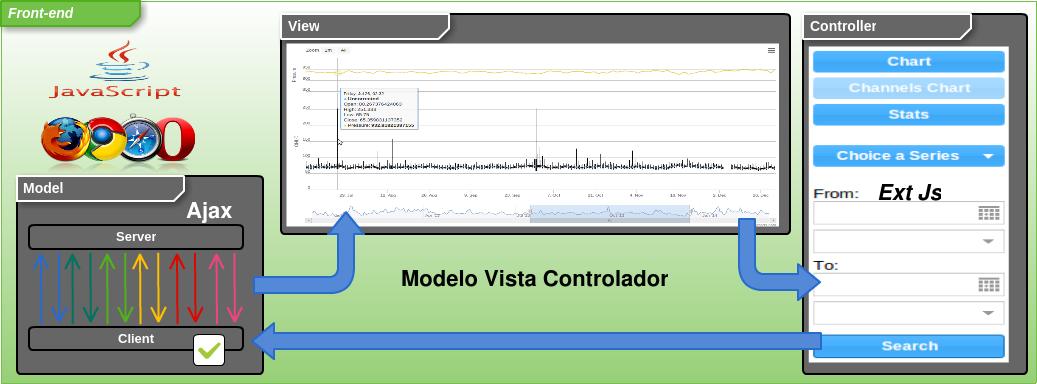
\includegraphics[keepaspectratio, width=1\textwidth]{./img/frontend.png}
	\caption{\emph{Front-end}. Patrón MVC.}   
	\label{fig:frontend}
\end{figure}
\section{Sencha ExtJs}
	El propósito de esta sección es explicar alguno de los aspectos básicos del framework. Empezaremos explicando como crear una aplicación básica
	basándonos en ExtJs. En la mayoría de los casos existe un solo documento HTML\cite{HTML} que contiene toda la aplicación. En este documento
	tenemos que cargar dos \emph{scripts} de la siguiente forma.
    		\begin{center} \texttt{<script type="text/javascript" src=\textquotedbl extjs/ext-all-debug.js\textquotedbl ></script>}  \end{center}
    		\begin{center} \texttt{<script type="text/javascript" src=\textquotedbl app.js\textquotedbl ></script>}  \end{center}
 	El primer \emph{script} contiene el framework que queremos utilizar. Es conveniente destacar que esta es una versión concebida para el proceso
	de desarrollo. Para la versión final es conveniente usar el \texttt{ext-all.js}.
 	\par
 	El segundo \emph{script} es el que contiene la lógica de nuestra aplicación. A continuación podemos ver el código mínimo para crear una
	aplicación. El código presentado será explicado a fondo.
	\begin{lstlisting}
Ext.application({
   name: 'HelloExt',
   launch: function() {
      Ext.create('Ext.container.Viewport', {
         layout: 'fit',
            items: [{
               title: 'Hello Ext',
               html : 'Hello! Welcome to Ext JS.'}] 
      }); 
   } 
});
	\end{lstlisting}
 	En la primera línea hacemos uso del singletone \texttt{Ext}. Este es un objeto que encapsula todas las clases, métodos y singletones
	proporcionados por el framework. La función utilizado \texttt{Ext.application} carga e inicializa una instancia de la clase
	\texttt{Ext.app.Application}. Esta clase representa una aplicación ExtJs single page. La llamada a esta función crea la variable global
	\texttt{MyApp}, que debe contener todas las clases e instancias de nuestra aplicación.
 	\par
 	En la segunda línea declaramos el nombre de nuestra aplicación. Seguidamente definimos la función \texttt{launch}. Esta es la función que debe
	lanzar  nuestra aplicación. La primera función invocada es \texttt{Ext.create} que crear una instancia de la clase proporcionada, en este caso
	\texttt{Ext.container.Viewport}. \texttt{Viewport} es un \emph{contenedor} que representa el área de aplicación y puede haber tan solo uno por
	aplicación. 
 	\par
 	La interfaz de usuario en una aplicación ExtJs es compuesta por \emph{componentes}. Un \emph{contenedor} es un \emph{componente} especial que
	contiene otros \emph{componentes}. En la figura \ref{fig:comps} podemos ver un ejemplo que ilustra esta jerarquía.
	\begin{figure}[h]
		\centering
		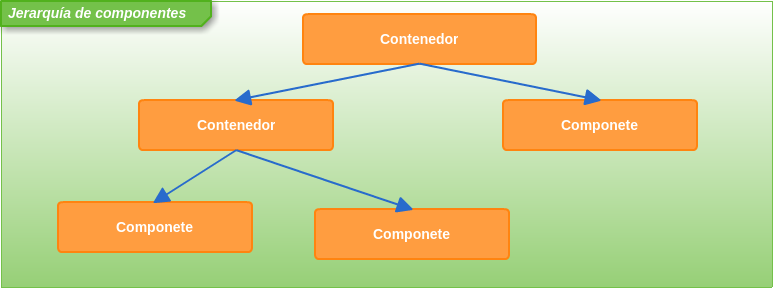
\includegraphics[keepaspectratio, width=1\textwidth]{./img/comps.png}
		\caption{Sencha ExtJs. Jerarquía de componentes.}   
		\label{fig:comps}
	\end{figure}
 	\par
 	El \texttt{Viewport} es el \emph{contenedor} que contiene todos los demás \emph{componentes} de nuestra aplicación. Los \emph{compenentes} de
	un \emph{contenedor} se especifican en el campo \texttt{items} que es una lista. En el ejemplo presentado tan solo tenemos un 
	\emph{conponente}, pero pueden ser añadidos más.
 	\par
 	Fijándonos en el código de ejemplo podemos ver antes de definir el campo \texttt{items} definimos el campo \texttt{layout}. El \texttt{layout}
	especifica la forma en la que se posicionaran y ajustaran los \emph{componetes} hijos. En este caso el \texttt{layout} especificado es 
	\texttt{\cc fit\cc} en el que un solo hijo ocupa todo el espacio del padre. 

\section{\emph{Modelo}}
	El \emph{modelo} es el encargado de manejar los datos de una aplicación. En el caso del \emph{front-end} los datos de la aplicación deben ser
	servidos por el \emph{back-end}. El \emph{modelo} es el encargado de realizar la comunicación con el \emph{back-end}. 
	\par
	Tal y como especificamos en el  capítulo anterior el protocolo para la comunicación entre los dos módulos es \emph{HTTP}. Nuestro
	\emph{front-end} es el que empieza la comunicación enviando un mensaje de petición y el \emph{back-end} responde a esa peticion con un mensaje
	de respuesta. El \emph{modelo} es el encargado de construir y enviar los mensajes de petición y después interpretar los mensajes de respuesta.
	\par
	Para dotar el \emph{modelo} de la funcionalidad necesaria vamos a ayudarnos de las facilidades que nos ofrece ExtJs, concretamente vamos a
	utilizar el singletone \texttt{Ext.Ajax}. Ajax\cite{AjaxWiki} es una técnica de desarrollo Web donde cliente y servidor mantienen una
	comunicación asíncrona en segundo plano. \texttt{Ext.Ajax} es un singletone de la clase \texttt{Ext.data.Connection}, clase que encapsula la
	lógica necesaria para realizar una comunicación Ajax. 
	\par
	Concretamente vamos a hacer uso de la función \texttt{Ext.data.Connection.request}. Esta función envía una petición \emph{HTTP} a un servidor
	remoto. La función acepta un solo parámetro que es un objeto cuyas propiedades definen el comportamiento de la función. Las propiedades de las
	que nosotros haremos uso están detalladas a continuación. 
	\begin{itemize}
  		\item	\texttt{url}. 	La URL a la que enviaremos la petición. En nuestro caso \emph{back-end} y \emph{front-end} estarán albergados en
		  	el mismo \emph{host}. Esto nos permite no especificar el \emph{host}, la petición se hará al \emph{host} utilizado para cargar
			la aplicación. En la URL tan solo tendremos que especificar el servicio deseado y los parámetros que acompañan a este.
			Seguidamente presentamos un ejemplo del valor que puede tomar el campo \texttt{url}.
    				\begin{center} \texttt{url: \cc/nmdadb/cannel/stats/default/default\cc}  \end{center}
		\item	\texttt{method}. El método que especifica nuestro mensaje de petición. Los mensajes \emph{HTTP} de petición pueden especificar
		  	un método. Si este campo es dejado vacío el método utilizado será \texttt{GET}. La mayoría de los servicios ofrecidos por el
			\emph{back-end} aceptan un método \texttt{GET}, pero el servicio \texttt{nmdbMarkNull} acepta un método \texttt{POST}.
		\item	\texttt{success}. La función a ser llamada al completar exitosamente la petición. Esta función a su vez acepta como parámetro
		  	\texttt{response}. Este parámetro contiene los datos del mensaje de respuesta.
		\item	\texttt{failure}. La función a ser llamada al completar sin éxito la petición. Esta función también acepta el parámetro
		  	\texttt{response} que podemos utilizar para identificar la causa del fallo.
		\item	\texttt{timeout}. El numero de milisegundos en los que el \emph{back-end} debe responder. Si el tiempo expira la solicitud se
		  	considera como fallida. 
	\end{itemize}
	Más allá de \emph{Ext.data.Connection} el framework ofrece abstracciones de un nivel superior. La clase \emph{Ext.data.Model} es una
	representación de un objeto utilizado por nuestra aplicación. Estos modelos son usados por la clase \emph{Ext.data.Store}, que encapsula
	instancias de un modelo. La clase \emph{Ext.data.Store} también hace uso del \emph{Ext.data.proxy.Proxy}, abstracción que permite cargar y
	guardad datos de un modelo. 
	\par
	Estas abstracciones son muy útiles, pero algo complejas. Al no estar acostumbrado a trabajar con ellas el autor de este trabajo ha preferido
	utilizarlas lo menos posible. Por esta razón la mayoría de los datos se manejan usando el \texttt{Ext.data.Connection}, hemos utilizado el
	\texttt{Ext.data.Store} en casos muy específicos.
